\documentclass[letterpaper,10pt,notitlepage,fleqn]{article}

%\usepackage{nopageno} %gets rid of page numbers
\usepackage{alltt}                                           
\usepackage{float}
\usepackage{color}
\usepackage{indentfirst}
\usepackage{url}
\usepackage{balance}
\usepackage[TABBOTCAP, tight]{subfigure}
\usepackage{enumitem}
\usepackage{pstricks, pst-node}
\usepackage{geometry}
\geometry{textheight=9in, textwidth=6.5in} %sets 1" margins 
\newcommand{\cred}[1]{{\color{red}#1}} %command to change font to red
\newcommand{\cblue}[1]{{\color{blue}#1}} % ...blue
\usepackage{hyperref}
\usepackage{textcomp}
\usepackage{listings}
\usepackage{graphicx}

\def\name{Sam Quinn}

\parindent = 0.4444 in
\parskip = 0.2 in

\begin{document}
\begin{titlepage}
\vspace*{\fill}

\newcommand{\HRule}{\rule{\linewidth}{0.5mm}} % Defines a new command for the horizontal lines, change thickness here

\center % Center everything on the page

%----------------------------------------------------------------------------------------
%TITLE SECTI   ON
%----------------------------------------------------------------------------------------

%\includegraphics[scale=.5]{image.eps}
\HRule \\[0.4cm]
{ \huge \bfseries Intel Flight Controller}\\[0.4cm] % Title of your document

%----------------------------------------------------------------------------------------
%HEADING SECTIONS
%----------------------------------------------------------------------------------------

\textsc{\LARGE IFC+}\\[0.5cm] % Name of your university/college
\textsc{\Large CS406 Special Project}\\[0.5cm] % Major heading such as course name
\textsc{\large Fall 2015}\\[0.5cm] % Minor heading such as course title


\HRule \\[1.5cm]
%----------------------------------------------------------------------------------------
%AUTHOR SECTION
%------------------------------------ ----------------------------------------------------

\begin{minipage}{0.4\textwidth}
\begin{flushleft} \large
\emph{Student:}\\
        \textbf{Sam \textsc{Quinn}} \\ % Your name
        {\small Quinnsa@Oregonstat.edu}
        \end{flushleft}
        \end{minipage}
        ~
        \begin{minipage}{0.4\textwidth}
        \begin{flushright} \large
        \emph{Mentor:} \\
            \textbf{Kevin \textsc{McGrath}} \\ % Supervisor's Name
            {\small D.Kevin.McGrath@Oregonstate.edu}
            \end{flushright}
            \end{minipage}\\[3cm]

            % If you don't want a supervisor, uncomment the two lines below and remove the section above
            %\Large \emph{Author:}\\
                %John \textsc{Smith}\\[3cm] % Your name

                %----------------------------------------------------------------------------------------
                %DATE SECTION
                %-----------------    -----------------------------------------------------------------------

{\large \today}\\[3cm] % Date, change the \today to a set date if you want to be precise

%----------------------------------------------------------------------------------------
%LOGO SECTION
%------   ----------------------------------------------------------------------------------

%\includegraphics{Logo}\\[1cm] % Include a department/university logo - this will require the graphicx package

%----------------------------------------------------------------------------------------

\vfill % Fill the rest of the page with whitespace



\end{titlepage}

\tableofcontents
\newpage

\section{Introduction}
\indent This Project was developed as an extracurricular for computer science elective credit.  The main goal of this project is to create a smarter flight controller. There are many flight controllers available today but none of them run on powerful hardware or have the expandable options that a full computer has. Our project is meant to use an Intel powered x86 microcomputer to replace the standard flight controller. With a powerful processor controlling the UAV we will be able
to expand the functionality to other useful features like video processing for object detection, wireless connectivity for WIFI traffic analysis, automated flight plans, and many other things. The core of this project is getting the UAV operable with standard components and connecting the peripherals to the Intel board.


\section{Platform}

\subsection{What platform did we decide to use?}
\indent During the initial stages of the project we wanted to use hardware that would be easy to setup and have decent developer community. With the nature of the project having to fly the ideal computer would be very small and lightweight. There a few Intel boards that we considered for this project. The Intel NUC, the Intel Galileo, the Intel Edison. The NUC is the biggest but has the most powerful hardware with an Intel i5. The Intel NUC is basically a 4x4 inch desktop computer.
The NUC would be able to perform other tasks with the excessive performance and would be a good choice for when we implement smart control. The Intel Galileo is the least powerful at processing but is designed with a breakout board built in. The Galileo would be the best for actually controlling the UAV peripherals since we could plug the components directly into the board itself. The Edison would be the Ideal board for this product since it bridges the gap between performance and breakout
capabilities. The Intel Edison has the smallest form factor that would be able to fit neatly on any size UAV and would be able to be powered directly from the 5V output from the ESCs.
\\
\indent We decided to start development on the Intel NUC in the early stages of development with plans to eventually develop on the Edison. This decision came from the idea that we first need to get Ardupilot running on the NUC which is an x86 computer. Almost all of the flight controllers out there today are on the ARM architecture we figured once we understand how to get Ardupilot running on a x86 architecture we will be able to transition it the other Intel boards at a later time.

\subsection{Other platforms}
\textbf{BeagleBone + Erle-Brain} \\
\indent The BeagleBone is a tiny credit card size Linux computer. This fully featured computer sports a quad-core Cortex-A7 and 512MB of ram which would easily take care of flight and leave enough processing power for other computations. For the BeagleBone to actually pilot the UAV and control the necessary hardware on board the Pixhawk Fire Cape cape comes into play. The Pixhawk Fire Cape adds all the necessary hardware to the base BeagleBone,
including;
\begin{itemize}
    \item 3-axis gyroscope
    \item 3-axis accelerometer
    \item 3-axis magnetometer
    \item Barometer
\end{itemize}
\indent On the software side of things the BeagleBone is able to run any ARM distribution of Linux including Debian and Ubuntu. The images that are recommend to use for this particular setup with the Erle-Brain are minimal server images, “snappy core” in Ubuntu or a distribution with the RT\_PREEMPT kernel patches. The snappy core or RT patches allow the BeagleBone to run in a soft real time state which is very important in aviation. 
\\ \\
\textbf{Pixhawk} \\
\indent While the Pixhawk flight controller is a prebuilt board the what interesting aspect here is the Nuttx operating system. The NuttX OS is open-source released under BSD license and real time by default. What makes NuttX OS so enticing is that it has a very small footprint, uses many POSIX standard OS interfaces, multi-threaded and real-time fully preemptible. NuttX has a large support for various platforms including ARM, MIPS, AVR, and what I really need for our Intel based flight
controller x86. 
\\ \\
\textbf{Co-Processor} \\
\indent One option proposed is to setup a co-processing computer. This would allow us to use a prebuilt flight controller that would be connected to a Intel computer. The computer would not need to actually ever calculate pitch, roll, yaw, GPS, motor control, or really anything to allow the UAV to fly. All the computer would do is take this data in the form of telemetry and process it. With the Intel board not needing to run a real-time OS it could function with an off the shelf Linux distro.
The Linux board would then be able to process data such as video for self driving or object avoidance and send the results back to the flight controller for actual control of the vehicle. The Linux co-processor would open up the opportunity to remotely control the UAV via WiFi or Cellular as sort of a man in the middle type setup. The problem with this setup is that it requires more stuff, more stuff means more weight. A lot of computers, even credit card size computers out there today
have more than enough processing power to run an entire UAV themselves without the need for a flight controller co-processor combo. 

\subsection{Considerations}
\indent The main problem when looking at the options listed above was the fact that they often deterred from our main goal to use an Intel based board. Main of the Linux tutorials on-line were based on very specific hardware and almost all were ARM architecture. APM had a Linux cross compile section but seemed very sparse in documentation and even littler developer community. The main reason I suspect that there is not much x86 development going on in the UAV world is that for a
while x86 computers were large, costly, and often do not have many IO options.
\section{Hardware}

\subsection{MultiRotor}
\indent For our actual UAV we decided to just build a standard quad-copter. I have had first hand experience building quad-copters before and feel comfortable with the design. Having only 4 motors to control individually reduces the number of IO ports necessary to get the vehicle off the ground. One of the things that we had to take into account was weight. We had to make sure that whatever development board we decided to use was able to be lifted by the hardware we chose.
An average 450 quad-copter equipped with 4 980kv motors has a maximum payload capacity of around 3 pounds. The UAV would start to feel sluggish after around 12,000g which is around 2.5lbs. The largest board that we proposed as a development option is the Intel NUC which weighed in at 478g about 1.05lbs with its heat sink case. We decided that the Intel i5 version of the NUC would suffice for all of the applications we wanted to develop for. With the heat generated from normal
operation we assumed (not tested) that if we removed the motherboard form the heavy heat sink case that the air would adequately cool the NUC on the UAV making the UAV much lighter. 

\subsection{Power}
\indent Powering a standard UAV can take varying voltages depending on the number of cells within the Lithium Polymer battery. Usually multi-rotors that are larger than 250 do not dip below 11.1v (3s) and can reach all the way up to 22.2v (6s). Many of the small ARM based flight controller projects that I have come across use a common 5v to power up the entire Linux computer. A 5v input power is very nice on a UAV because many of the ESCs will down convert the Li-Po battery to a
manageable 5v by default to power things like the flight controllers or radio receivers. Powering a thing like an Intel NUC is something different since it takes 19.5v DC. There are step down converters that will manage a 6s Li-Po battery and convert the 22v to 19.5v, but that adds an extra piece of a hardware. 

\subsection{Rx Radio Receiver}
\indent Two of the most common communication protocols via radio transmission are PPM (Pulse Position Modulation) and PWM (Pulse Width Modulation). Each are very different with PPM being the newer protocol. PWM requires a cable for each individual channel and needs very accurate widths to function properly. PPM needs only one cable to output the same amount of data. Most of the tutorials I found on-line use PPM and I think for good measure. 
\\
\indent Reading in PPM from a radio Rx receiver, the system absolutely needs a real-time unit. To get accurate data from the Rx the computer must pull the pins very quickly and consistently for long periods of time without any hiccups. To pull these pins to receive Tx data is almost impossible to do in Linux user-space. With a hypervisor like QUEST we could technically use one of the cores of the i5 to be dedicated real-time and load a real-time OS only for that core. If we could get the
QUEST hypervisor running properly we could use that as our PRU (Programmable Real-time Unit). This PRU would not need to ever execute anything that would strain the one core it just would need to have a really reliable clock tick, since that is how PPM is determined where the position of the pulse is at. 

\subsection{Telemetry}
\indent Telemetry is much simpler on a Linux computer than many flight controllers today. Since a Linux computer is designed for users to access the internet they have WiFi and or USB ports that would allow wireless data to be transmitted, flight controllers don't. The most popular telemetry transmission client is MAVLink (Micro Aerial Vehicle Link) that will work with GCS (Ground Control Station). MAVLink is able to send telemetry data via UART, UDP, or TCP. UDP
seems like the best choice since the Intel flight controller would either have WiFi built in or  could be easily added. UDP is also a non guaranteed delivery protocol so if the UAV ever went out of the range of WiFi, not too far, it would not halt the transmission. When the UAV would return to connecting distance it would simply pick up what the current state is at the moment without having to resend all the lost packets.

\subsection{Connectivity}
\indent With many of the prototyping boards available today connectivity is usually not a problem. One of the things that make the small prototyping boards that have been ported to APM ideal is that they often times have built in UARTs, I2C, or SPI connectivity. The problem with using the Intel NUC is that it does not have these peripheral interfaces. The Intel NUC does however have USB connections which we will be able to connect something like an FPGA. A FPGA connect
via USB would be able to take in inputs form sensors and send out PWM outputs to the ESCs. With the many uses that an FPGA would add it seems like a good fit for the limited connectivity of the Intel NUC. I was not aware of vast amount of uses that FPGAs offer, there have been UAVs that have been fully programed with only a FPGA.

\section{Software}

\subsection{HyperVisor}
\indent With the luxury of having a powerful multi-core processor controlling our UAV we will have a lot of processing power left over. Having a hypervisor to control sub-operating systems is a great way to separate the systems software components. The baseline processing power to actually control a UAV in aerial flight does not require much hardware. The idea to isolate one core of the Intel NUC and run a sand-boxed standalone OS such as ROS or NuttX is great. This type of setup
would allow the 3 remaining cores to still continue to run a Linux OS and have user-space applications run in conjunction, allowing the one isolated core run in real-time controlling the UAV in a reliable environment.
\\
\indent Quest is a multi-kernel sand-boxing tool that allows complete separation of cores. The separation of the cores are allowed to run complete operating systems due to the creation of a virtual CPU on the isolated core. Quest actually bootstraps the isolation at startup without having to trust the hypervisor to manage the resources at runtime. Having the bootstrapping makes this system very reliable throughout power cycles and could very well be implemented in a UAV. 
\\ 
\indent With priorities we would be able to create a fairly stable soft-real-time system with isolating cores using Quest and is depicted below. \\
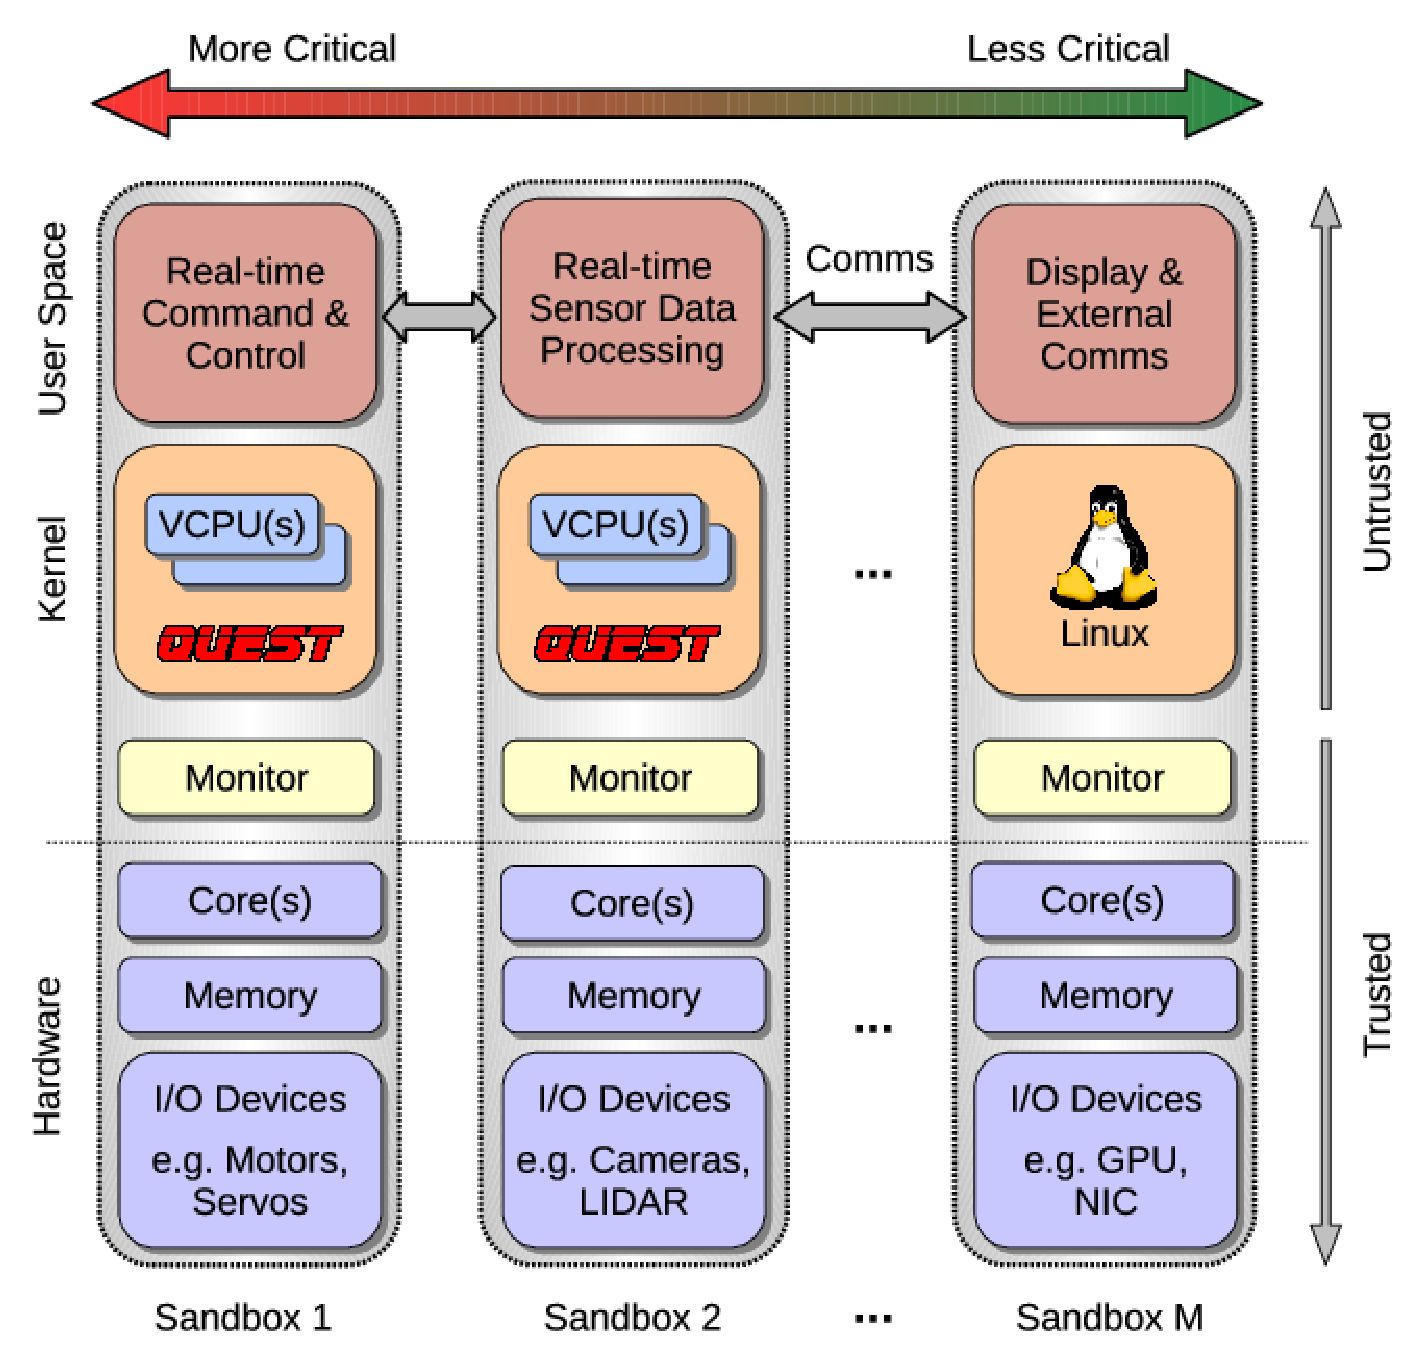
\includegraphics[scale=.5]{quest-v-overview.eps} \\
Quest-V is a configurable virtualized multi-kernel hypervisor that is able to take advantage of direct hardware virtualization features to form a collection of separate kernels with individual name-spaces. Quest-V is perfect for a project like this because we never want any errors to cause disruption to the underlying flying functionality. Quest-v uses virtualization techniques that isolate each individual kernel which prevents localized faults from affecting any of the other isolated
kernels. 

\subsection{ROS}
\indent ROS stands for Robotic Operating System and is a repository based OS with modular features. You are able to pick and choose which features you will need and leave the rest uninstalled. ROS allows for crucial libraries to be linked for an UAV to function including message passing, localization, preemptable procedure calls, mapping, navigation, and diagnostics. ROS is a middleware application that provides a great interface when porting APM to a x86 Linux implementation. While ROS is
not designed specifically for multi-rotors the open source community has opened many opportunities for fully autonomous flight. 
\\
\indent There have been multiple modules implemented for ROS that bridge the gap between the APM flight code and the ROS operating system. Because ROS is a repository based system users are able to create packages that are imported through ROS for easy integration. MAVLink as described above is a way for the UAV to communicate flight data with external applications. ROS is able to take advantage of the MAVLink telemetry bridge with the mavlink\_ros package that creates
a serial MAVLink connection to the ROS system. Mavlink\_ros in conjunction with the roscopter package we are actually able to directly communicate through the MAVLink serial bridge and control the autopilot by overriding the RC input commands. Through my research the mavros package  would be one of the most feature rich packages and would be best suited for this particular project. mavros is able to communicate via UDP, TCP, or serial to the autopilot, create a UDP GCS
proxy, update mission and way-points, and mavros can act as a failsafe safety tool. 

\subsection{Simulation Software}
\indent One of the very useful tools that I discovered while doing my research is the SITL (Software In The Loop) simulator. SITL allows you to compile unmodified Ardupilot code directly from the source and test it in a virtual environment. This was nice for this project's early stages since you are able to test all the software without the need for any hardware. The simulator adds all the same functionality to the virtual UAV that you would get from the real craft. The
simulator is also able to simulate your flying environment with adjustable wind speed and direction. 
SITL is able to connect to an either virtual or real UAV with the MAVLink protocol either with MAVProxy (UDP) or without MAVProxy (TCP). With the simulator we are able to test our software implementations with Quest and ROS and determine if the real-time execution is adequate without putting live hardware at risk of a crash. The picture below shows the relationships between each component.  
\\
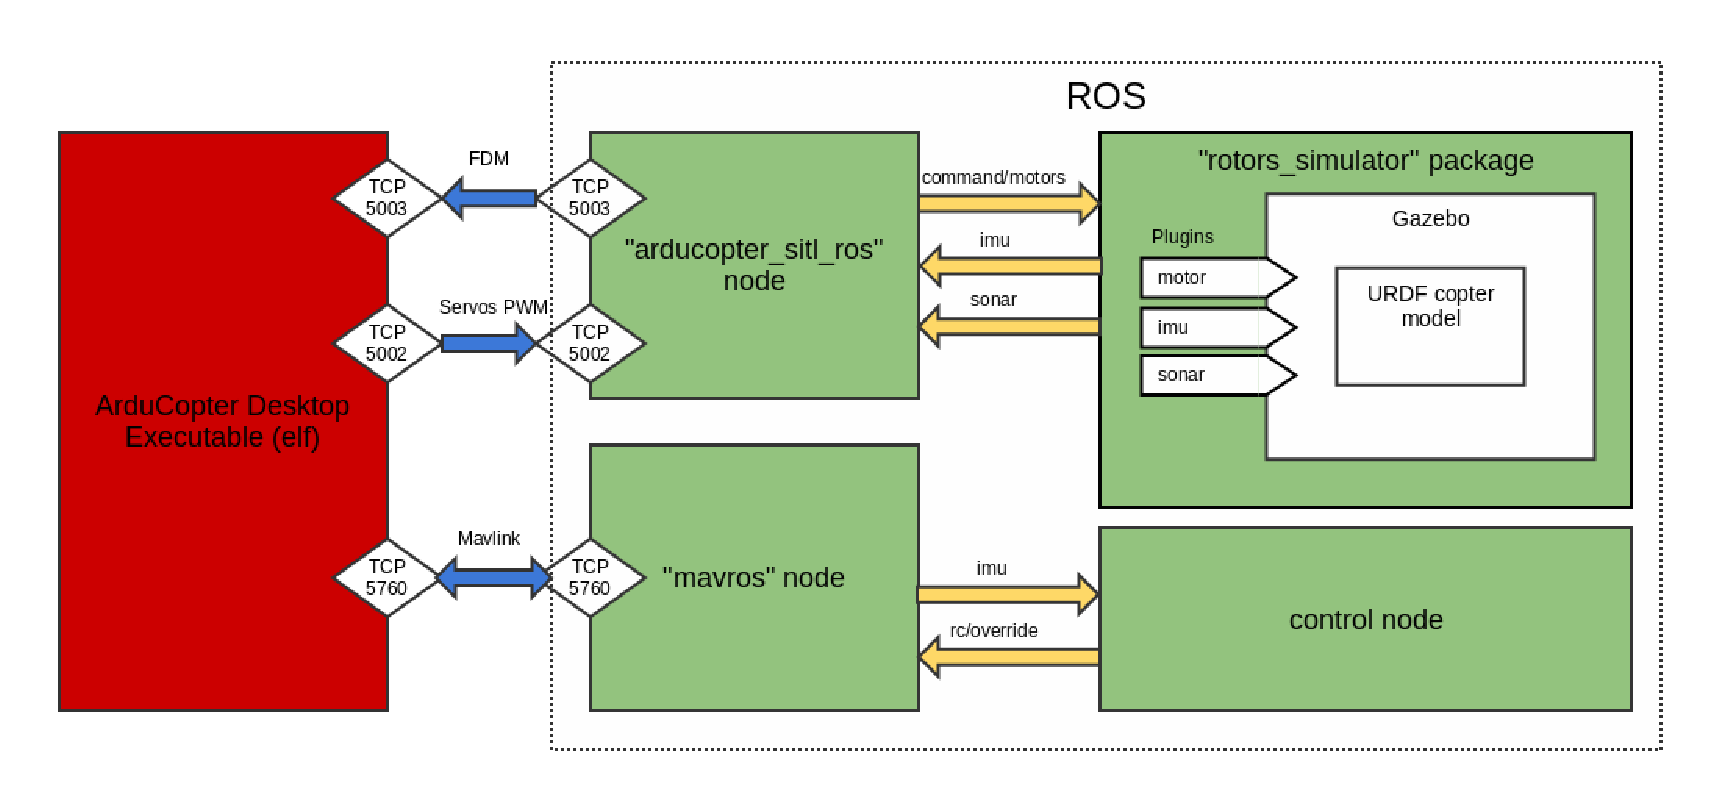
\includegraphics[scale=.5]{arducopter_sitl_ros.eps} \\
This picture does not show the implementation of the Quest hypervisor which would have the ROS chunk running in a completely sand-boxed kernel environment, while the Ardupilot could be either running in the same sandbox or a separate sandbox. 

\section{Conclusion}
\subsection{What I learned}
\indent I have been building and flying quad-copters for a round a year now and always thought that the system was fairly simple. After this project I see that to create your own flight controller the software and hardware is much more intricate than I thought. While there was not much documentation on Ardupilot running on Linux there was almost none in regards to Ardupilot running on a x86 Linux machine. Because the lack of documentation to reference for x86 Linux it was a
lot of trial and error. I would often times get hung up on getting each individual component to compile and worse run. Many of the software aspects of this project besides Ardupilot were not intentionally made to run UAV code. While there were many ports and plugins for ROS and Quest, the flight controller I was trying to create with the Intel based board was one of a kind. Because it was not as simple as downloading a complete suite or a binary I had a difficult time getting
all of the aspects to work with each other. 
\subsection{How this project benefited me}
\indent This project introduced me to the often overlooked part of the UAV hobby. I would have never dove this far down into any of the code that controls my quad-copter without this project as inspiration. I now understand how UAV embedded software within the hardware is setup and gives me a greater knowledge base for the UAV hobby. I have never had to use a real-time scheduler for any other project before and was great to see the benefits. Learning the uses of a real-time
scheduler and understanding what it means to be preemptable is great knowledge that I can take to other embedded projects. 
\\
\indent While researching this project it was the first time that I felt like I was doing something that not many others have accomplished. School projects are often reused problems that have been solved time and time again but building your own Intel flight controller is very unique. I would have to find documentation or write-ups that pertained to something completely different than I was working on and try to morph the process to my needs. Most of the source code was written for ARM base
processors so I got better at cross-compiling and reading compile errors. 
One thing I really liked learning was how PPM and PWM work. I know that PWM is used in many other functions including dimming LEDs but I have always been curious as to how data from the RC controller would be sent. I also learned how PPM and PWM is not possible without a very accurate and consistent clock tick which is often only available in a real-time environment. PPM was even more interesting on how even just the position of a pulse can be used to transmit data. I
understand why PPM outputs with only one cable since it serializes the received input.

\subsection{What still needs to be done}
\indent The work that I have done on this project has been mostly research. I have not yet gotten a working implementation of ROS or Quest on the Intel NUC. I was able to run the Ardupilot copter code on the Intel NUC in a SITL environment. The OS I decided to use on the NUC was Arch Linux since I thought that it would be easy to implement new features using the AUR package interface with ties to Github. I was able to install ROS and mavros package but was never able to link it to
the Ardupilot Copter code. The one thing that I really wanted was the Quest hypervisor to work. I downloaded the source code and followed the instructions to compile but was never able to get it to compile correctly. I was fairly disappointed to find out that the newest version of Quest was V1.0 which lead me to believe that the project was either non-maintained or abandoned. I also setup a virtual machine on the Oregon State network that is able to successfully run a
Ardupilot in a SITL environment. I was able to experiment with MAVLink commands through the MAVLink console. 
\\ 
\indent For this project to continue we must first iron out the software before we begin throwing hardware in the mix. Quest needs to be setup for the hypervisor to allow isolation of the real-time and user-space applications. We also will need to get the hardware figured out to be able to read in RC data as well as output PWM to control the ESCs and the motors. For future visions of the project we will be able to take advantage of ROS modular packages to implement computer vision
and autopilot, but these are implementations that can be added later.   

\subsection{Problems I came accross}
\indent There were a lot of problems that I came across in while working on this project. One of the most common problem I would come across was the lack of documentation. I would often find interesting pieces of software that would benefit the project, while they would say they support x86 Linux they would not provide the documentation. Quest was the worst at this, it was very hard to find any documentation that explaining the installation process. I downloaded the source
code and could not get past the compelling stage. 
\\
\indent ROS was documented but it was still a difficult system to get to understand. The documentation that I ran across while researching the external packages were very advanced and hard to follow. I was able to get ROS installed on my Arch Linux computer and able to install the roscopter, mavlink\_ros, and mavros. After installation there were configurations that I was not able to get to communicate with the simulated UAV. The reason that I did not dive deeper into this
issue was because I never actually was able to setup Quest to give ROS a real-time running environment. It was frustrating getting certain aspects to work but not being able to tie all of them together. 

\end{document}
